% Options for packages loaded elsewhere
\PassOptionsToPackage{unicode}{hyperref}
\PassOptionsToPackage{hyphens}{url}
%
\documentclass[
]{article}
\usepackage{amsmath,amssymb}
\usepackage{iftex}
\ifPDFTeX
  \usepackage[T1]{fontenc}
  \usepackage[utf8]{inputenc}
  \usepackage{textcomp} % provide euro and other symbols
\else % if luatex or xetex
  \usepackage{unicode-math} % this also loads fontspec
  \defaultfontfeatures{Scale=MatchLowercase}
  \defaultfontfeatures[\rmfamily]{Ligatures=TeX,Scale=1}
\fi
\usepackage{lmodern}
\ifPDFTeX\else
  % xetex/luatex font selection
\fi
% Use upquote if available, for straight quotes in verbatim environments
\IfFileExists{upquote.sty}{\usepackage{upquote}}{}
\IfFileExists{microtype.sty}{% use microtype if available
  \usepackage[]{microtype}
  \UseMicrotypeSet[protrusion]{basicmath} % disable protrusion for tt fonts
}{}
\makeatletter
\@ifundefined{KOMAClassName}{% if non-KOMA class
  \IfFileExists{parskip.sty}{%
    \usepackage{parskip}
  }{% else
    \setlength{\parindent}{0pt}
    \setlength{\parskip}{6pt plus 2pt minus 1pt}}
}{% if KOMA class
  \KOMAoptions{parskip=half}}
\makeatother
\usepackage{xcolor}
\usepackage{longtable,booktabs,array}
\usepackage{calc} % for calculating minipage widths
% Correct order of tables after \paragraph or \subparagraph
\usepackage{etoolbox}
\makeatletter
\patchcmd\longtable{\par}{\if@noskipsec\mbox{}\fi\par}{}{}
\makeatother
% Allow footnotes in longtable head/foot
\IfFileExists{footnotehyper.sty}{\usepackage{footnotehyper}}{\usepackage{footnote}}
\makesavenoteenv{longtable}
\usepackage{graphicx}
\makeatletter
\def\maxwidth{\ifdim\Gin@nat@width>\linewidth\linewidth\else\Gin@nat@width\fi}
\def\maxheight{\ifdim\Gin@nat@height>\textheight\textheight\else\Gin@nat@height\fi}
\makeatother
% Scale images if necessary, so that they will not overflow the page
% margins by default, and it is still possible to overwrite the defaults
% using explicit options in \includegraphics[width, height, ...]{}
\setkeys{Gin}{width=\maxwidth,height=\maxheight,keepaspectratio}
% Set default figure placement to htbp
\makeatletter
\def\fps@figure{htbp}
\makeatother
\setlength{\emergencystretch}{3em} % prevent overfull lines
\providecommand{\tightlist}{%
  \setlength{\itemsep}{0pt}\setlength{\parskip}{0pt}}
\setcounter{secnumdepth}{-\maxdimen} % remove section numbering
\ifLuaTeX
  \usepackage{selnolig}  % disable illegal ligatures
\fi
\IfFileExists{bookmark.sty}{\usepackage{bookmark}}{\usepackage{hyperref}}
\IfFileExists{xurl.sty}{\usepackage{xurl}}{} % add URL line breaks if available
\urlstyle{same}
\hypersetup{
  hidelinks,
  pdfcreator={LaTeX via pandoc}}

\author{}
\date{}

\begin{document}

\hypertarget{dataset-summary}{%
\subsection{Dataset Summary}\label{dataset-summary}}

The dataset,
\href{https://www.kaggle.com/datasets/rakeshkapilavai/extrovert-vs-introvert-behavior-data?resource=download}{Introverts
\& Extroverts}, contains 2900 entries and 8 columns.

\textbf{Dataset Information:}

\begin{verbatim}
<class 'pandas.core.frame.DataFrame'>
RangeIndex: 2900 entries, 0 to 2899
Data columns (total 8 columns):
 #   Column                     Non-Null Count  Dtype  
---  ------                     --------------  -----  
 0   Time_spent_Alone           2837 non-null   float64
 1   Stage_fear                 2827 non-null   object 
 2   Social_event_attendance    2838 non-null   float64
 3   Going_outside              2834 non-null   float64
 4   Drained_after_socializing  2848 non-null   object 
 5   Friends_circle_size        2823 non-null   float64
 6   Post_frequency             2835 non-null   float64
 7   Personality                2900 non-null   object 
dtypes: float64(5), object(3)
memory usage: 181.4+ KB
\end{verbatim}

\textbf{Column Descriptions:}

\begin{itemize}
\tightlist
\item
  \textbf{Time\_spent\_Alone}: Hours spent alone daily (0--11).
\item
  \textbf{Stage\_fear}: Presence of stage fright (Yes/No).
\item
  \textbf{Social\_event\_attendance}: Frequency of social events
  (0--10).
\item
  \textbf{Going\_outside}: Frequency of going outside (0--7).
\item
  \textbf{Drained\_after\_socializing}: Feeling drained after
  socializing (Yes/No).
\item
  \textbf{Friends\_circle\_size}: Number of close friends (0--15).
\item
  \textbf{Post\_frequency}: Social media post frequency (0--10).
\item
  \textbf{Personality}: Target variable (Extrovert/Introvert).
\end{itemize}

\hypertarget{data-exploration-plan}{%
\subsection{Data Exploration Plan}\label{data-exploration-plan}}

\begin{enumerate}
\def\labelenumi{\arabic{enumi}.}
\tightlist
\item
  Calculate the summary statistics for the numerical features. This
  includes mean, median, mode, std, min, max, and quartiles to
  understand the distribution of variables.
\item
  Generate box plots for all numerical fields to visually understand the
  distribution and summary statistics.
\item
  Generate pairplots. Pairplots will visualize relationships between all
  numerical features, colored by the `Personality' target variable, to
  identify potential patterns.
\item
  Generate a correlational heatmap. A correlational heatmap will
  quantify the linear relationships between numerical features, helping
  to identify highly correlated variables. This will be generated for
  each of the two personality types to find patterns specific to
  Extroverts and Introverts.
\end{enumerate}

\hypertarget{exploratory-data-analysis-eda}{%
\subsection{Exploratory Data Analysis
(EDA)}\label{exploratory-data-analysis-eda}}

\hypertarget{summary-statistics}{%
\subsubsection{1. Summary Statistics}\label{summary-statistics}}

\begin{longtable}[]{@{}
  >{\raggedright\arraybackslash}p{(\columnwidth - 10\tabcolsep) * \real{0.1038}}
  >{\raggedright\arraybackslash}p{(\columnwidth - 10\tabcolsep) * \real{0.1698}}
  >{\raggedright\arraybackslash}p{(\columnwidth - 10\tabcolsep) * \real{0.2358}}
  >{\raggedright\arraybackslash}p{(\columnwidth - 10\tabcolsep) * \real{0.1415}}
  >{\raggedright\arraybackslash}p{(\columnwidth - 10\tabcolsep) * \real{0.1981}}
  >{\raggedright\arraybackslash}p{(\columnwidth - 10\tabcolsep) * \real{0.1509}}@{}}
\toprule\noalign{}
\begin{minipage}[b]{\linewidth}\raggedright
Statistic
\end{minipage} & \begin{minipage}[b]{\linewidth}\raggedright
Time\_spent\_Alone
\end{minipage} & \begin{minipage}[b]{\linewidth}\raggedright
Social\_event\_attendance
\end{minipage} & \begin{minipage}[b]{\linewidth}\raggedright
Going\_outside
\end{minipage} & \begin{minipage}[b]{\linewidth}\raggedright
Friends\_circle\_size
\end{minipage} & \begin{minipage}[b]{\linewidth}\raggedright
Post\_frequency
\end{minipage} \\
\midrule\noalign{}
\endhead
\bottomrule\noalign{}
\endlastfoot
count & 2837.00 & 2838.00 & 2834.00 & 2823.00 & 2835.00 \\
mean & 4.51 & 3.96 & 3.00 & 6.27 & 3.56 \\
std & 3.48 & 2.90 & 2.25 & 4.29 & 2.93 \\
min & 0.00 & 0.00 & 0.00 & 0.00 & 0.00 \\
25\% & 2.00 & 2.00 & 1.00 & 3.00 & 1.00 \\
50\% & 4.00 & 3.00 & 3.00 & 5.00 & 3.00 \\
75\% & 8.00 & 6.00 & 5.00 & 10.00 & 6.00 \\
max & 11.00 & 10.00 & 7.00 & 15.00 & 10.00 \\
\end{longtable}

We observe that the standard deviation is significantly skewed for all
fields (abs(skew) \textgreater{} 0.75).

\hypertarget{box-plot}{%
\subsubsection{2. Box Plot}\label{box-plot}}

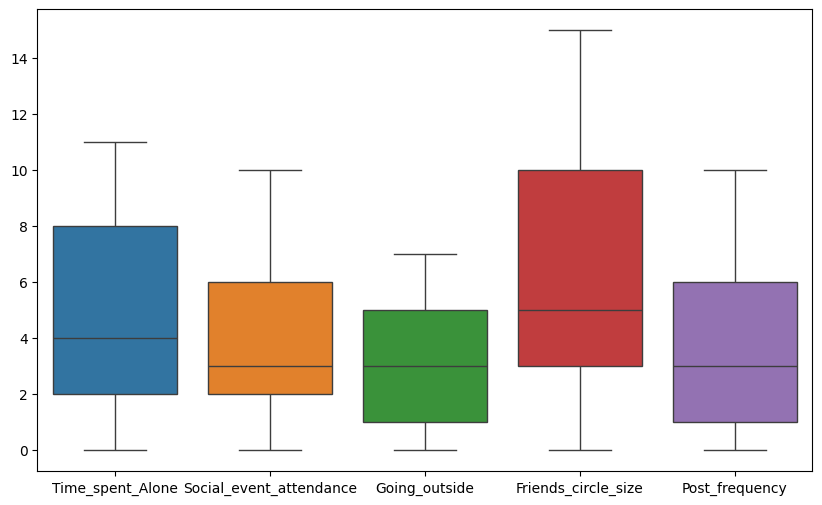
\includegraphics{3_2.png}

We don't observe any outliers, which makes sense since our metrics are
bounded for all fields.

\hypertarget{pairplots}{%
\subsubsection{3. Pairplots}\label{pairplots}}

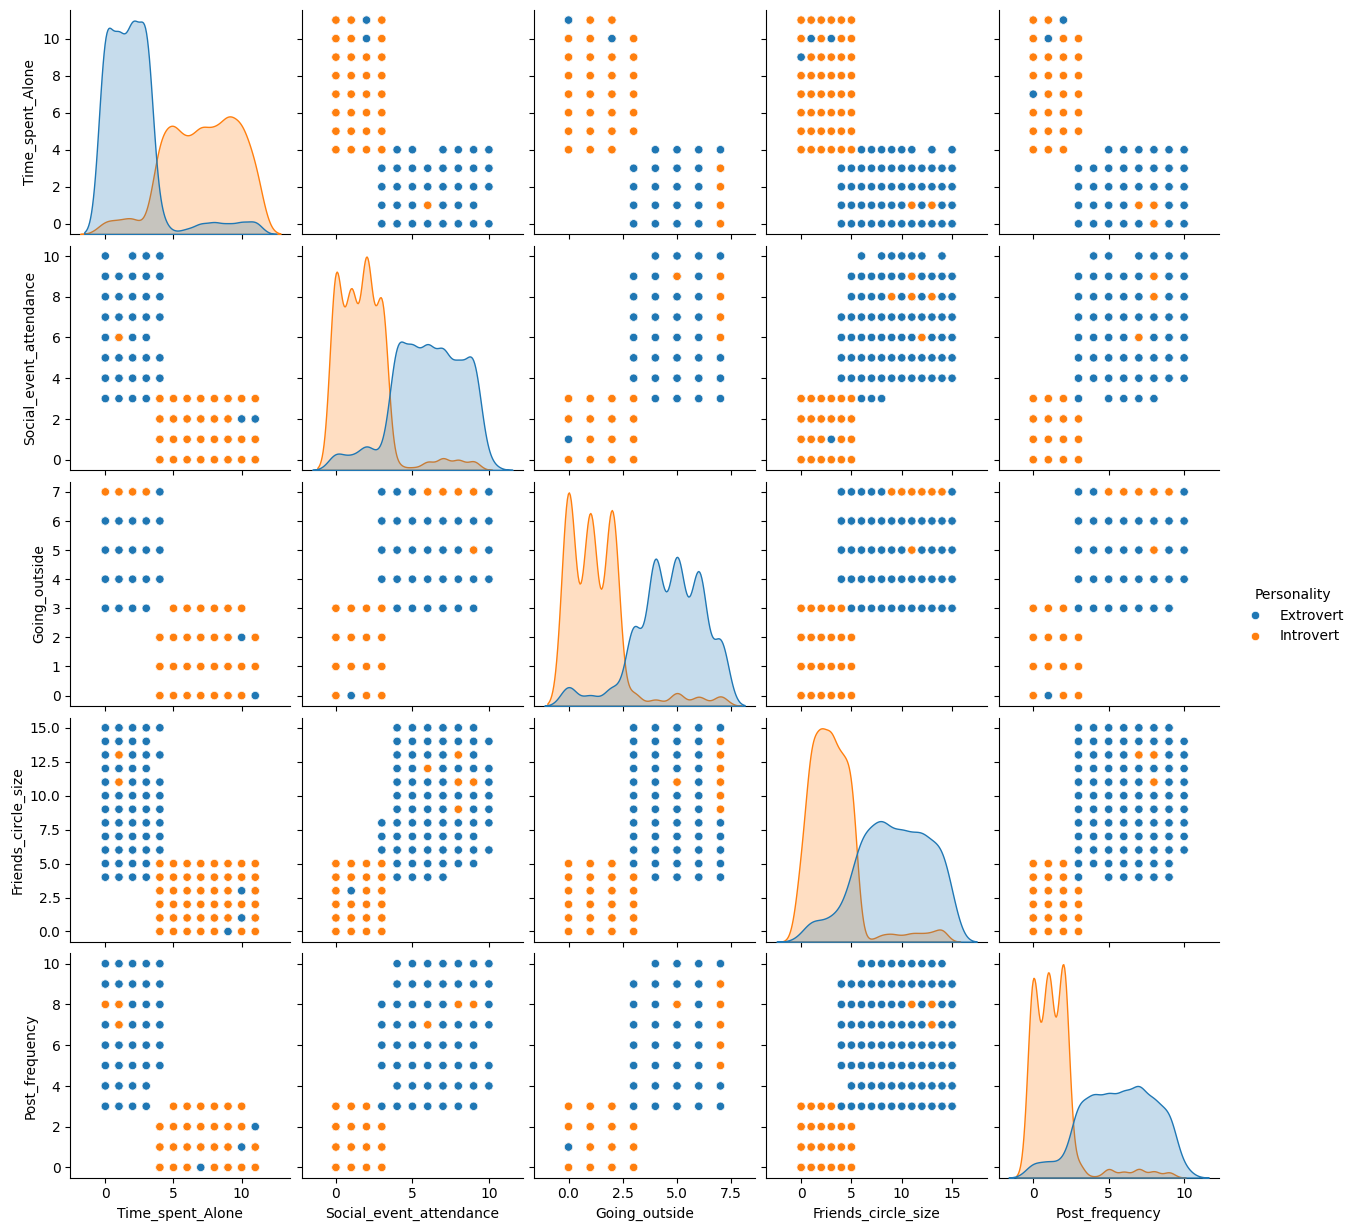
\includegraphics{3_3.png}

We see that for all features there exists a significant clustering
separating the introverts from the extroverts, this tells us that the
KNN algorithm could help significantly with predicting the target. We
also notice that most features are highly correlated.

\hypertarget{correlational-heatmap}{%
\subsubsection{4. Correlational Heatmap}\label{correlational-heatmap}}

Correlational Heatmap

\begin{figure}[htbp]
    \centering
    \begin{minipage}[t]{0.48\textwidth}
        \centering
        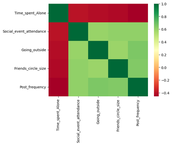
\includegraphics[width=\textwidth]{3_4_1.png}
        Introverts
    \end{minipage}
    \hfill
    \begin{minipage}[t]{0.48\textwidth}
        \centering
        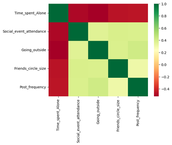
\includegraphics[width=\textwidth]{3_4_2.png}
        Extroverts
    \end{minipage}
\end{figure}

We observe that features are more correlated for introverts than
extroverts. \textbf{Time\_spent\_Alone} is a significant indicator for
both extroverts and introverts.

\hypertarget{data-cleaning-and-feature-engineering}{%
\subsection{Data Cleaning and Feature
Engineering}\label{data-cleaning-and-feature-engineering}}

\begin{enumerate}
\def\labelenumi{\arabic{enumi}.}
\item
  The null values that in this dataset encompus almost every column and
  there is no simple pattern to fill them, we could do knn. but if we
  dropp all rows with null values, we then remain with 2477 entries,
  which means we removed 423 entries. This isn't a significant, so we'll
  be going with that approach
\item
  We'll be log transforming the numerical fields to fix the skew and
  have normally distributed data, we'll be using log1p since we can have
  values of 0
\item
  We'll be using binary encoding for the fields \textbf{Stage\_fear},
  \textbf{Drained\_after\_socializing} and \textbf{Personality}

  \begin{longtable}[]{@{}
    >{\raggedright\arraybackslash}p{(\columnwidth - 14\tabcolsep) * \real{0.1224}}
    >{\raggedright\arraybackslash}p{(\columnwidth - 14\tabcolsep) * \real{0.0816}}
    >{\raggedright\arraybackslash}p{(\columnwidth - 14\tabcolsep) * \real{0.1701}}
    >{\raggedright\arraybackslash}p{(\columnwidth - 14\tabcolsep) * \real{0.1020}}
    >{\raggedright\arraybackslash}p{(\columnwidth - 14\tabcolsep) * \real{0.1837}}
    >{\raggedright\arraybackslash}p{(\columnwidth - 14\tabcolsep) * \real{0.1429}}
    >{\raggedright\arraybackslash}p{(\columnwidth - 14\tabcolsep) * \real{0.1088}}
    >{\raggedright\arraybackslash}p{(\columnwidth - 14\tabcolsep) * \real{0.0884}}@{}}
  \toprule\noalign{}
  \begin{minipage}[b]{\linewidth}\raggedright
  Time\_spent\_Alone
  \end{minipage} & \begin{minipage}[b]{\linewidth}\raggedright
  Stage\_fear
  \end{minipage} & \begin{minipage}[b]{\linewidth}\raggedright
  Social\_event\_attendance
  \end{minipage} & \begin{minipage}[b]{\linewidth}\raggedright
  Going\_outside
  \end{minipage} & \begin{minipage}[b]{\linewidth}\raggedright
  Drained\_after\_socializing
  \end{minipage} & \begin{minipage}[b]{\linewidth}\raggedright
  Friends\_circle\_size
  \end{minipage} & \begin{minipage}[b]{\linewidth}\raggedright
  Post\_frequency
  \end{minipage} & \begin{minipage}[b]{\linewidth}\raggedright
  Personality
  \end{minipage} \\
  \midrule\noalign{}
  \endhead
  \bottomrule\noalign{}
  \endlastfoot
  1.609438 & 0 & 1.609438 & 1.945910 & 0 & 2.639057 & 1.791759 & 0 \\
  2.302585 & 1 & 0.000000 & 0.000000 & 1 & 0.000000 & 1.386294 & 1 \\
  2.302585 & 1 & 0.693147 & 1.098612 & 1 & 1.791759 & 1.098612 & 1 \\
  0.000000 & 0 & 1.945910 & 2.079442 & 0 & 2.708050 & 2.197225 & 0 \\
  1.386294 & 0 & 2.302585 & 1.609438 & 0 & 2.197225 & 1.791759 & 0 \\
  \end{longtable}
\item
  Using PCA we can explain 99\% of the variance with 2 principle
  components, dropping our feature count from 7 to 2
\end{enumerate}

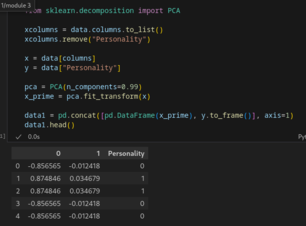
\includegraphics{4_4.png}

\hypertarget{key-findings-and-insights}{%
\subsection{Key Findings and Insights}\label{key-findings-and-insights}}

\begin{itemize}
\tightlist
\item
  \textbf{Personality Clustering}: Pairplots revealed distinct
  clustering between introverts and extroverts across all features,
  indicating that these features are strong predictors of personality
  type. This suggests that algorithms like K-Nearest Neighbors (KNN)
  could be highly effective for personality prediction.
\item
  \textbf{Feature Correlation Patterns}: Features exhibited stronger
  correlations for introverts compared to extroverts. This difference in
  correlation patterns between the two personality types is a
  significant insight.
\item
  \textbf{``Time\_spent\_Alone'' as a Key Indicator}: The feature
  ``Time\_spent\_Alone'' was identified as a significant indicator for
  both extroverts and introverts, highlighting its importance in
  distinguishing between the two personality types.
\item
  \textbf{Dimensionality Reduction Effectiveness}: Through PCA, it was
  discovered that 99\% of the dataset's variance could be explained by
  just two principal components. This indicates that the data can be
  effectively represented in a much lower dimension while retaining
  almost all its information, which is crucial for model efficiency and
  interpretability.
\end{itemize}

\hypertarget{hypothesis-formation}{%
\subsection{Hypothesis Formation}\label{hypothesis-formation}}

\begin{enumerate}
\def\labelenumi{\arabic{enumi}.}
\tightlist
\item
  The mean post frequency is more for introverts than extroverts.
\item
  There isn't a significant difference for people having stage fright
  between introvers and extroverts
\item
  The mean size of an extrovert's friend circle is larger than an
  introvert's.
\end{enumerate}

\hypertarget{hypothesis-testing-significance-analysis}{%
\subsection{Hypothesis Testing \& Significance
Analysis}\label{hypothesis-testing-significance-analysis}}

We are going to be testing: The mean post frequency is more for
introverts than extroverts. The intuition being that since introverts
spend more time on their own, they are more likely to spend more time
online which could mean they post more.

\begin{itemize}
\item
  Our null hypothesis (\(H_0\)): the mean post frequency for introverts
  is more than extroverts (\(\mu_{introvert} > \mu_{extrovert}\))
\item
  Our alternative hypothesis (\(H_A\)): the mean post frequency for
  extroverts is equal to or more than introverts
  (\(\mu_{extrovert} \ge \mu_{introvert}\))
\end{itemize}

Since we have a contrasting hypothesis, we'll be using the
Neyman-Pearson Interpretation of \(H_0\) and \(H_1\).

We'll be setting our significance level \(\alpha = 5\%\).

Since we don't know the standard deviation for the population, we'll be
using a t-test since we have a large sample size.

The `\textless{}' sign in the alternative hypothesis indicates the test
is left-tailed.

\hypertarget{introvert-distribution}{%
\subsubsection{Introvert Distribution}\label{introvert-distribution}}

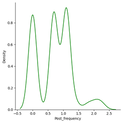
\includegraphics{7_1.png}

\hypertarget{extrovert-distribution}{%
\subsubsection{Extrovert Distribution}\label{extrovert-distribution}}

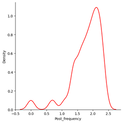
\includegraphics{7_2.png}

\begin{itemize}
\tightlist
\item
  \(\mu_{introvert} = 0.71\)
\item
  \(\mu_{extrovert} = 1.79\)
\item
  \(t = -51.5\)
\item
  \(p = 0.0\)
\end{itemize}

Looking at the density distribution, we can already get a strong
indicator that our null hypothesis is false. Doing further calculation
on the mean values, we can see that \(\mu_{extrovert}\) is a whole page
frequency more, and finally, doing the test, we get a p-value of 0,
which is below our significance level of 5\%. So it is clear we can
reject our null hypothesis and quite confidently state that extroverts
post more frequently than introverts.

\hypertarget{conclusion-next-steps}{%
\subsection{Conclusion \& Next Steps}\label{conclusion-next-steps}}

\hypertarget{key-takeaways}{%
\subsubsection{Key Takeaways:}\label{key-takeaways}}

\begin{itemize}
\tightlist
\item
  \textbf{Personality Prediction}: The dataset features are strong
  predictors of personality type, with distinct clustering observed
  between introverts and extroverts. This suggests that machine learning
  algorithms like K-Nearest Neighbors (KNN) could be highly effective
  for personality prediction.
\item
  \textbf{Feature Importance}: ``Time\_spent\_Alone'' is a significant
  indicator for both personality types, highlighting its importance in
  distinguishing between introverts and extroverts.
\item
  \textbf{Dimensionality Reduction}: PCA effectively reduced the
  dataset's dimensionality, explaining 99\% of the variance with just
  two principal components. This is crucial for building efficient and
  interpretable models.
\item
  \textbf{Hypothesis Testing}: The hypothesis test regarding post
  frequency clearly indicates that extroverts post more frequently than
  introverts, with a p-value of 0, allowing us to confidently reject the
  null hypothesis.
\end{itemize}

\hypertarget{next-steps}{%
\subsubsection{Next Steps:}\label{next-steps}}

\begin{itemize}
\tightlist
\item
  \textbf{Model Building}: Develop and train a machine learning
  classification model (e.g., KNN, Logistic Regression) to predict
  personality type based on the processed features.
\item
  \textbf{Data Splitting}: Split the dataset into training and testing
  sets to validate the generalization of our model.
\item
  \textbf{Model Training}: Train the chosen machine learning model on
  the training data.
\item
  \textbf{Model Evaluation}: Evaluate the trained model's performance on
  the testing data using appropriate metrics.
\end{itemize}

\end{document}
